\documentclass[11pt,final]{article}
\usepackage{a4wide}
\usepackage{color}
\usepackage{graphicx}
\usepackage{listings}
\usepackage{hyperref}
\usepackage{array}
\usepackage{xspace}
\usepackage{comment}

\setlength{\parindent}{0pt}
\setlength{\parskip}{5pt}

\definecolor{lightgray}{rgb}{.95,.95,.95}
\definecolor{middlegray}{rgb}{.55,.55,.55}
\lstset{
  basicstyle=\footnotesize\ttfamily,
  keywordstyle=\bfseries\ttfamily,
  commentstyle=\color{middlegray}\ttfamily,
  tabsize=2,
  numbers=none,
  numberstyle=\tiny,
  numberblanklines=false,
  stepnumber=1,
  numbersep=10pt,
  language=bash,
  xleftmargin=0pt,
  backgroundcolor=\color{lightgray}
}

\newcommand{\Gt}[0]{\emph{GenomeTools}\xspace}
\newcommand{\Gtj}[0]{\emph{GenomeTools-Java}\xspace}
\newcommand{\FO}[0]{\emph{FISH Oracle}\xspace}


\title{The \FO user manual}
\author{Malte Mader, Sascha Steinbi\ss}

\begin{document}

\maketitle
\tableofcontents

\section{Introduction}

This user manual describes how to install, configure and maintain the
\FO software. To get a first impression of the software visit
\url{http://www.zbh.uni-hamburg.de/fishoracle} to watch a screencast video or
try out a demo installation.
We also offer a virtual machine with an
already set up \FO application which provides a quick and easy way to
use a private instance of \FO. If you want to use \FO
collaboratively in production mode we encourage to set up a private
installation at an own machine. Due to the technical limitations of
virtual machines (slow, little storage) its use for large amounts of
data is not recommendable.

\subsection{Requirements and Availability}

To be able to install and run \FO, the following software packages are
needed along with their individual dependencies:

\begin{itemize}
  \item MySQL database server
  \item Apache Tomcat server (requires Java JRE)
  \item \Gt with MySQL support (requires Cairo library)
  \item \FO (requires Java JDK and ant)
\end{itemize}

If you want to install Tomcat or MySQL manually, you can download it from
\url{http://tomcat.apache.org/} and \url{http://www.mysql.com/downloads/mysql}
respectively. This is only necessary if you do not have administration rights
on the system you want to install \FO.
\Gt is available for download from \url{https://github.com/genometools/genometools}.
\Gtj and \FO can be obtained from \url{http://www.zbh.uni-hamburg.de/fishoracle} or
\url{https://github.com/mader}.

\begin{comment}

\section{Installation}

\subsection{Linux -- Debian 6.0}
\label{debian}

\subsubsection*{Installing the prerequisites}

An installation script for the automatic installation of all needed software
packages and the \FO software is provided at
\url{http://www.zbh.uni-hamburg.de/fileadmin/gi/FISHOracle/install_fishoracle_debian.sh}.
The script needs to be executed with administration rights.

If you want to install the needed software manually open a terminal.
In case you are using the Gnome desktop, simply open a terminal using the GNOME
menu (Applications $\rightarrow$ Accessories $\rightarrow$ Terminal) and
execute the following commands as root:

\begin{lstlisting}

> echo deb http://ftp.de.debian.org/debian squeeze main \
 contrib non-free >> /etc/apt/sources.list

> apt-get update

> apt-get install mysql-server sun-java6-jdk

> echo 'JAVA_HOME="/usr/lib/jvm/java-6-sun"' >> /etc/environment
> echo 'JRE_HOME="/usr/lib/jvm/java-6-sun/jre"' >> /etc/environment

> export JAVA_HOME="/usr/lib/jvm/java-6-sun"

> apt-get install ant tomcat6 libcairo2-dev libncurses5-dev
\end{lstlisting}

\subsubsection*{Installing \FO}

To set up the actual \FO application, proceed to sections \ref{db-setup}
(Database setup) and \ref{fo-install} (\FO installation).

\end{comment}

\subsection{Linux -- Ubuntu 12.04 LTS}
\label{ubuntu}

\subsubsection*{Installing the prerequisites}

An installation script for the automatic installation of all needed software
packages and the \FO software is provided at
\url{http://www.zbh.uni-hamburg.de/fileadmin/gi/FISHOracle/install_fishoracle_ubuntu.sh}.
The script needs to be executed with administration rights (e.g.\ using
\texttt{sudo}).

If you want to install the software manually, open a terminal
and execute the following commands (you may be prompted for your password):

\begin{lstlisting}
> sudo apt-get install python-software-properties

> add-apt-repository ppa:webupd8team/java

> sudo apt-get update

> sudo apt-get oracle-java7-installer

> echo 'JAVA_HOME=/usr/lib/jvm/java-7-oracle' >> /etc/environment
> echo 'JRE_HOME=/usr/lib/jvm/java-7-oracle/jre' >> /etc/environment

> export JAVA_HOME="/usr/lib/jvm/java-7-oracle"

> sudo apt-get install mysql-server ant tomcat libcogl-pango-dev\
 libcairo2-dev libncurses5-dev libmysqlclient-dev ruby libmysql-ruby\
 git
\end{lstlisting}

\subsubsection*{Installing \FO}

To set up the actual \FO application, proceed to sections \ref{db-setup}
(Database setup) and \ref{fo-install} (\FO installation).

\subsection{Mac OS X 10.6 -- Snow Leopard}
\label{macosx}

\subsubsection*{Installing the prerequisites}

To install \FO on a Mac server, prior installation of the Apple Developer
Tools is required to obtain a development environment ready to compile C and
Java source code. The Developer Tools should be included on separate media with
along the system software of every Mac system. This software package should
also contain the \emph{ant} software needed to build \FO. Please install the
Developer Tools in the usual way from the Apple media.

To install the necessary Cairo library as an additional dependency,
we recommend to use the Fink software package system
(\url{http://www.finkproject.org}).
For more information on how to do this, please refer to the Fink documentation
(e.g.\ \url{http://www.finkproject.org/download/index.php} for a quick start).

After successful Fink installation, open a terminal
(Applications $\rightarrow$ Utilities $\rightarrow$ Terminal)
and execute the following commands:

\begin{lstlisting}
 > sudo /sw/bin/fink -b install cairo
\end{lstlisting}

Also, \FO uses MySQL to store annotation information, user accounts and
other data to be visualized. MySQL can be installed via Fink, but we recommend
getting a Mac OS X version from the official MySQL download site
(\url{http://dev.mysql.com/downloads/mysql}). The easiest option is to choose
the \texttt{.dmg} file, mount it and follow the installation instructions in
the file \texttt{ReadMe.txt}.


\subsubsection*{Installing \FO}

As Apache Tomcat is not available in the Fink repository, get a Tomcat
``core'' distribution from the Apache download page
(\url{http://tomcat.apache.org/download-60.cgi}). We recommend the
\texttt{tar.gz} version. Then, unpack it in a directory of your choice:

\begin{lstlisting}
 > tar -xzvf apache-tomcat-6.0.32.tar.gz
\end{lstlisting}

This results in a new directory \texttt{apache-tomcat-6.0.32} being created.
The contents of this directory can now be moved or copied to any desirable
location on the server. The destination will be further referred to as the
``Tomcat installation directory''.

To set up the actual \FO application, proceed to sections \ref{db-setup}
(Database setup) and \ref{fo-install} (\FO installation).

\section{Database setup}
\label{db-setup}

This section explains how to set up the database for use with \FO and how to
import annotation data. Note that prior to this step you should have created a
user account in the MySQL system for exclusive use with \FO. In the following
examples, we will refer to this account as \texttt{<mysql\_user>} and to the
associated password as \texttt{<mysql\_password>}. Please consult the MySQL
documentation or your system administrator for more information about how to
set up a MySQL user account.

\subsection{Ensembl database}

Download the genome annotation data of your choice from the Ensembl FTP server.
The current version of \FO supports all Ensembl versions between 54
and 72. For example, to retrieve the annotations from Ensembl release 72,
download from \url{ftp://ftp.ensembl.org/pub/release-72/mysql}.

For instance, to download the human genome annotation execute the following
command in a terminal:

\begin{lstlisting}
> wget -r -nd ftp://ftp.ensembl.org/pub/release-72/mysql/homo_sapiens_core_72_37
\end{lstlisting}

Create a database, unpack all tar files and import the SQL schema and data
into the database:

\begin{lstlisting}
> mysql -u <mysql_user> -p
mysql> CREATE DATABASE ensembl;

> mysql -u <mysql_user> -p ensembl < homo_sapiens_core_72_37.sql

> mysqlimport -u <mysql_user> -p --fields_escaped_by=\\ \
   ensembl -L *.txt
\end{lstlisting}

\subsection{\FO database}

Create a \FO database. Download the source code for the \FO database API from
\url{https://github.com/mader/fishoracle_db_api}. The easiest way is to
execute the install script \texttt{install\_db.sh} which automatically
installs a \FO database named ``fishoracle'' containing an administration user
called ``admin'' with the password ``admin''.

If you want to install the database manually, import the SQL database schema
(\texttt{emptyoracle.sql}) plus initial data (\texttt{data.sql}) into the
\FO database:

\begin{lstlisting}
> wget http://www.zbh.uni-hamburg.de/fishoracle/fishoracle_db_api.tar.gz

> tar -xvzf fishoracle_db_api.tar.gz

> mysql -u <mysql_user>
mysql> CREATE DATABASE fishoracle;
mysql> USE fishoracle;
mysql> SOURCE fishoracle.sql;
\end{lstlisting}

\subsection{Setup initial user}

In the last installation step an initial user account for the \FO with
administration rights should be created. Open your browser, load the FISH
Oracle application and register a new user with your desired username, say
\emph{adminuser}. 

Next, open a terminal and login to the MySQL console and type the following
commands:

\begin{lstlisting}
mysql> use fishoracle;
mysql> update user set isactive = 1 where user.username = 'adminuser';
mysql> update user set isadmin = 1 where user.username = 'adminuser';
\end{lstlisting}

\section{\FO installation}
\label{fo-install}

For the installation of the \Gt you can use the installation script
\texttt{install\_geneomtools.sh} which is part of the \FO source code.

The last part of the installation is distribution independent
and therefore at every system the same. If the PC is a 64 bit
architecture the \Gt need to be compiled with the 64bit
flag. So make sure that in line 4 you use \texttt{make 64bit=yes}
instead of \texttt{make}.

\begin{lstlisting}

> wget http://www.zbh.uni-hamburg.de/fileadmin/gi/FISHOracle/fishoracle.tar.gz

> tar -xvzf fishoracle.tar.gz

> wget https://github.com/genometools/genometools/archive/master.zip

> tar -xvzf master.tar.gz

> cd master

> cp ../fishoracle/gt_db_api/* .

> make with-mysql=yes

> sudo make install

> cd ../fishoracle

\end{lstlisting}

Before compiling the \FO application, the database connections have
to be set up. The databases installation is explained in
chapter~\ref{db-setup}. The connections are specified in
\textit{war/config/database.conf}. The configuration parameters need to be
adapted to your database names and login specifications. The structure of the
file looks as follows:

\begin{verbatim}
[ensembl]

host = localhost
port = 3306
db = ensembl
user = <mysql_user>
pw = <mysql_password>

[fishoracle]

host = localhost
db = fishoracle
user = <mysql_user>
pw = <mysql_password>
\end{verbatim}

Finally the application can be compiled and copied to the Tomcat server.
Compilation is started by running \texttt{ant} with the \texttt{war} target:

\begin{lstlisting}
> ant war
\end{lstlisting}

If the compilation completed successfully, the resulting WAR file must be
put into the Tomcat webapps directory for deployment.
If you followed the Linux instructions (sections \ref{debian} and \ref{ubuntu}),
this is done by:

\begin{lstlisting}
> cp fishoracle.war /var/lib/tomcat6/webapps
\end{lstlisting}

Mac users simply copy the \texttt{fishoracle.war} file into the \texttt{webapps}
subdirectory of their Tomcat installation.

In the next step, it is necessary to start the Tomcat server. Linux users do
this with the following line:

\begin{lstlisting}
> /var/lib/tomcat6/bin/catalina.sh start
\end{lstlisting}

Mac users run the \texttt{bin/catalina.sh} script with the \texttt{start}
parameter in the subdirectory in which their Tomcat installation is located.

Now the \FO application should be accessible at
\url{http://localhost:8080/fishoracle}.

If any errors occur, a look at the files in the \texttt{log/} subdirectory of
the Tomcat installation may be helpful.

%\subsection{Install \Gt from source}

%\subsection{Install \Gtj from source}

%\subsection{Install Java manually}

%\subsection{Install Tomcat manually}

\section{Configuration}

\subsection{Data Import}

\subsubsection{File Formats}

New data is imported from tab delimited files. Depending on the datatype the
necessary data columns vary.


\paragraph{Copy Number Variation Data}

Following columns have to be present in order to import Copy Number Variation
(CNV) data:

\begin{enumerate}
  \item Chromosome column (``chr'')
  \item Start position (``start'')
  \item End position (``end loc'')
  \item Number of markers (``markers'')
  \item Segment mean intensity value (``segment mean'')
\end{enumerate}

Table \ref{tab:tsv_cnv} exemplifies the structure of a tab delimited CNV data file.

\begin{table}
	\centering
	\begin{tabular}[h]{|c|c|c|c|c|c|c|}
	  \hline
	 chr & start & end loc & markers & segment mean \\ \hline
	 1 & 10000 & 20000 & 135 & -0.27 \\
	 1 & 21000 & 25000 & 57 & 0.01 \\
	 1 & 25001 & 30000 & 80 & -0.3 \\
	 2 & 3000 & 5000 & 22 & 0.21 \\
	 2 & 8000 & 10000 & 15 & 0.28 \\
	 2 & 11000 & 18000 & 47 & 0.3 \\
	 \vdots & \vdots & \vdots & \vdots & \vdots \\
	\end{tabular}
	\caption{Structure of the tab delimited import files for CNV data}
	\label{tab:tsv_cnv}
\end{table}

\paragraph{Single Nucleotide Varoation Data}

Following columns have to be present in order to import Copy Number Variation
(CNV) data:

\begin{enumerate}
  \item Chromosome column (``\#CHROM'')
  \item SNV position (``POS'')
  \item dbSNP ID (``DBSNP\_ID'')
  \item Reference (``REF'')
  \item Alternative (``ALT'')
  \item Quality score (``QUAL'')
  \item Somatic or germline mutation (``SOMATIC\_GERMLINE\_CLASSIFICATION'')
  \item Confidence level (``CONFIDENCE'')
\end{enumerate}

\begin{table}
	\centering
	\begin{tabular}[h]{|c|c|c|c|c|c|c|c|}
	  \hline
	  \#CHROM & POS & DBSNP\_ID & REF & ALT & QUAL & {*}SGC & CONFIDENCE \\ \hline
	 1 & 10000 & rs55798854 & G & T & 75 & somatic & high confidence\\
         1 & 25001 & . & A & G & 66 & somatic & medium confidence\\
         1 & 3000 & rs12345678 & T & C & 25 & somatic & low confidence\\
         1 & 8000 & . & G & C & 120 & germline & high confidence\\
	\vdots & \vdots & \vdots & \vdots & \vdots & \vdots & \vdots & \vdots \\
	\end{tabular}
	\caption{Structure of the tab delimited import files for SNV data.
	{*}SOMATIC\_GERMLINE\_CLASSIFICATION}
	\label{tab:tsv_snv}
\end{table}

Table \ref{tab:tsv_snv} exemplifies the structure of a tab delimited SNV data file.

\paragraph{Translocation Data}

\paragraph{Generic Feature data}

\subsubsection{Web application import}

The data import comprises 2 steps: The upload of the tab delimited file and
the actual import of the data and meta data into the database.
After the upload the user needs to specify an appropriate microarray study
name. By default the file name is suggested. Furthermore the chip type and a
tissue need to be specified. Figure \ref{fig:import} depicts the data import.

\begin{figure}[h]
	\begin{center}
	  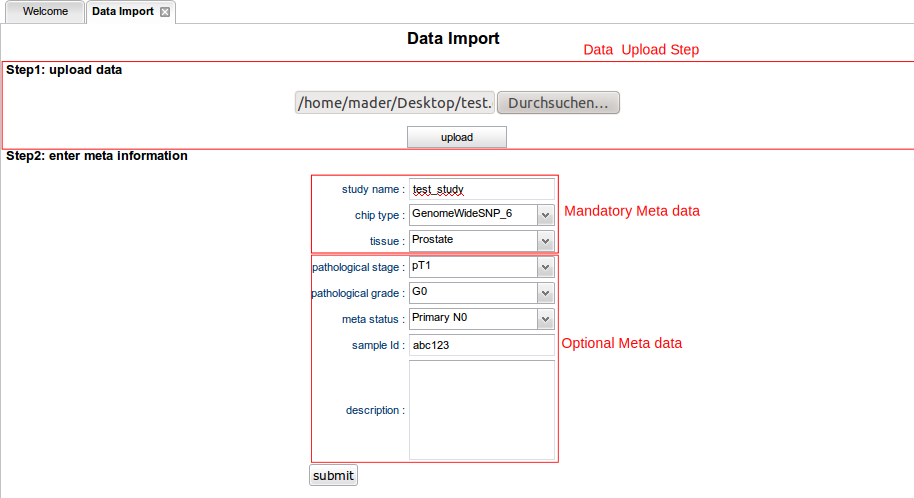
\includegraphics[width=\textwidth]{fig/import.pdf}
	\end{center}
	\caption{Screenshot of the import page.}
	\label{fig:import}
\end{figure}

%\subsubsection{FISH Oracle importer}

%\subsection{Run more than one \FO-Application on a Tomcat server}

\subsection{Database Connection}

The database connection can either be configured directly in the configuration
file in the subdirectory \texttt{webapps/fishoracle/war/config/database.conf}
located in the Tomcat main directory or, alternatively, directly in the web
application.
The changes take effect immediately after saving the changes in the file or
submitting the changes via the application. There is no need to restart the
Tomcat server or to recompile \FO. Figure \ref{fig:dbconfig}
illustrates the database configuration interface.

\begin{figure}[h]
	\begin{center}
		\includegraphics[width=\textwidth]{fig/dbconfig.png}
	\end{center}
	\caption{The database configuration interface provides the possibility
	         to change the database connection instantly.}
	\label{fig:dbconfig}
\end{figure}

\subsection{AnnotationSketch Visualization}

The appearance of the visualization can be influenced by a \emph{style file}
located in \textit{war/config/default.style}. The file contains Lua code that
is evaluated during the image rendering process. It includes display
definitions for genes, segment data, various genomic and non-genomic elements
as well as global display options corresponding to the spacing or visibility
of elements and captions. For detailed explanation of the style file see
\url{http://genometools.org/style_options.html}.

This section briefly summarizes the most important options to customize the
visualization of \FO.

The options for the display of segment data e.g. looks as follows:
\begin{verbatim}

cnc = {
    -- Color definitions
    stroke_marked      = {red=1.0, green=0.0, blue=0.0},
    style              = "box",
  },

\end{verbatim}

The option \textit{stroked\_marked} means in this example, that a found element
representing segment data will be marked with a red border. The option
\textit{style} determines that all elements will be drawn as a rectangular
box.

To get a more compact visualization captions of elements could be disabled
and spaces between tracks could be adapted:

\begin{verbatim}

show_block_captions = false, -- generally show captions
show_track_captions = false, -- generally show track captions

bar_vspace = 5,   -- space between feature bars, in pixels
track_vspace = 15, -- space between tracks, in pixels

\end{verbatim}

The display of captions for specific elements is also adjustable with the
\textit{max\_capt\_show\_width} option. The value is a threshold up to which
captions are shown. If the width of the displayed sequence region
(in characters) exceeds this value, then captions are omitted. If set to 0,
captions are never shown for this type. If set to \textit{nil}, then captions are
always shown.
The following example shows the option in the context of segment data where
captions are completely disabled.

\begin{verbatim}

cnc = {
    -- Color definitions
    stroke_marked      = {red=1.0, green=0.0, blue=0.0},
    style              = "box",
    max_capt_show_width= 0,
  },


\end{verbatim}

%\section{Usage}

\end{document}
